% CREATED BY DAVID FRISK, 2016
\chapter{Background}
\textit{In this chapter a general glance on Artificial Intelligence, and its sub-categories, is given.}\\\\

\epigraph{ \textit{Can a machine think?}}{--- \textup{Alan Turing}, Computing Machinery and Intelligence}

\section{Overview}
In the past decade many companies have started to advertise the use of AI, even if they are using a subfield of the AI, in their products and software applications. Nevertheless, the exponential growth of the last decade,
the AI is not youth.\\ It takes one of its roots from a theoretical paper of \textit{Alan Turing} published by journal \textit{Mind} in the 1950 \cite{paper:36}.\\

The general definition of Artificial Intelligence (AI) is intelligence demonstrated by machines, any device that perceives its environment and takes actions that maximize its chance of successfully achieving its goals.\\ In general, ''artificial intelligence'' is used when machines mimics the cognitive functions of the human mind, i.e. learning and problem solving.\\
According to the definition, AI is too vast to be studied and simulated. Therefore, it has been divided into subfields, characterized by different traits, such as knowledge representation, planning, learning, natural language processing, perception, motion and manipulation, social intelligence, general intelligence.\\\\

Artificial Intelligence can be seen as a general purpose technology. It does not exist a general task on which it excels neither how to characterize them.

\begin{figure}[H]
\centering
\captionsetup{justification=centering}
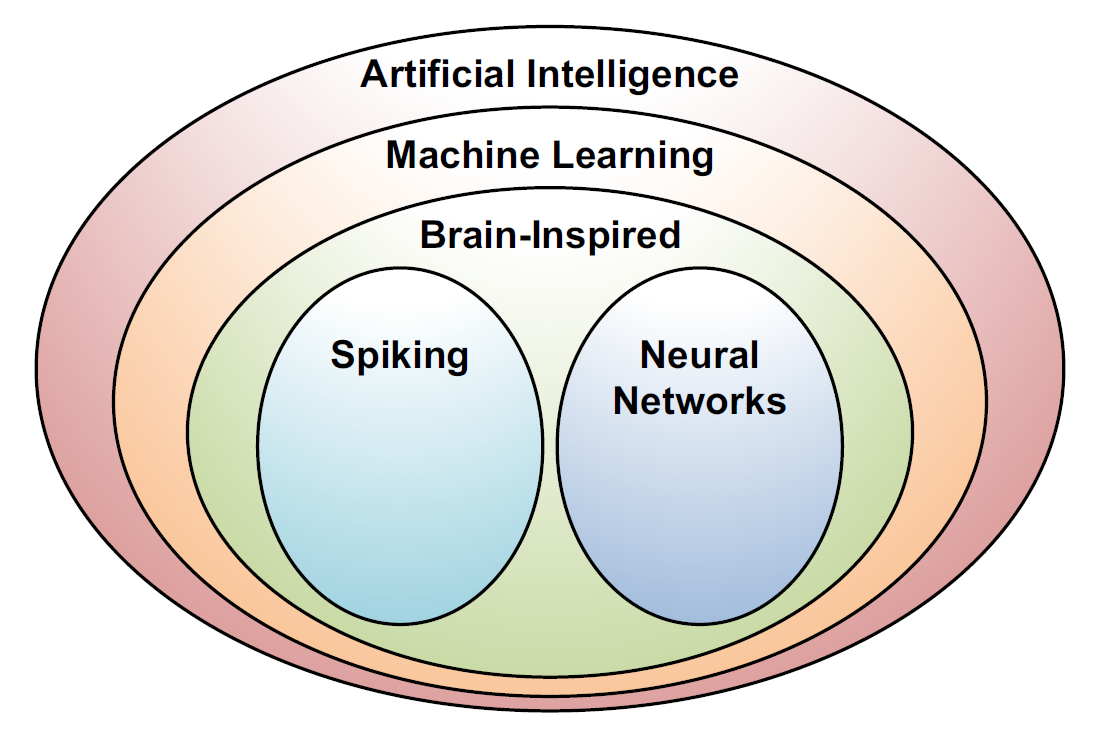
\includegraphics[scale=0.5]{./figure/ai_division.PNG}
\caption{Classification of AI with emphasis on Machine Learning and its subclassification}
\label{fig:aidiv}
\end{figure}

\section{Machine Learning}
A particular interesting subcategory of AI in Computer Science is the machine learning. It is the study of algorithms used to perform a specific task without explicit programming the machine, relying on patterns and inference, in order to make decisions. This approach is used where it is tricky, or unfeasible, to develop a conventional algorithm for solving the task.\\

A peculiarity of machine learning model is that it is composed of two processes, training and inference.\\
The inference process is the process in which a conclusion is given at the end of the evaluation process, i.e. the input stimulus are applied to the model and the output is observed.\\
The training process has to be done before the model is put on the field, before the inference process, otherwise the latter can give wrong results. As the name suggest, in this process the model learns how to behave, adjusting the weight accordingly to the applied inputs and expected outputs. Besides this type of training and according to \cite{book:1}, other exists, characterized by approach, type of data and tasks:
\begin{itemize}
\item Supervised Learning, it builds a mathematical model of a set of data that contains both the inputs and the desired outputs.
\item Unsupervised Learning, it takes a set of data that contains only inputs and find structure in the data.
\item Semi-supervised Learning, it falls between unsupervised learning and supervised learning.
\item Reinforcement Learning, it concerns how software agents should take actions in order to maximize some notion.
\item Self Learning, It is a learning with no external rewards and no external teacher advices.
\item Feature Learning, also called representation learning algorithms, often attempt to transform data and preserve at the same time, it is used as a preprocessing step before any classification or predictions.
\item Sparse Dictionary Learning, it is a feature learning method where a training example is represented as a linear combination of basis functions, and is assumed to be a sparse matrix.
\item Anomaly Detection, also known as outlier detection, 
the aim is to identify rare items, events or observarions which are significantly different from the majority of data.
\item Association Rules, it is a rule-based method for discovering relationships between variables in large databases.
\end{itemize}

Machine learning space is also divided into other type of models such as decision tree, support vector machines, regression analysis, bayesian networks and genetic algorithms.
As it can be seen in Figure \ref{fig:aidiv} Brain Inspired machine learning is also divided in subcategories.
\subsection{Brain Inspired}
It is based on algorithms which take its basic functionalities from our understanding of how the brain operates, trying to mimic the functionalities.

\begin{figure}[H]
\centering
\captionsetup{justification=centering}
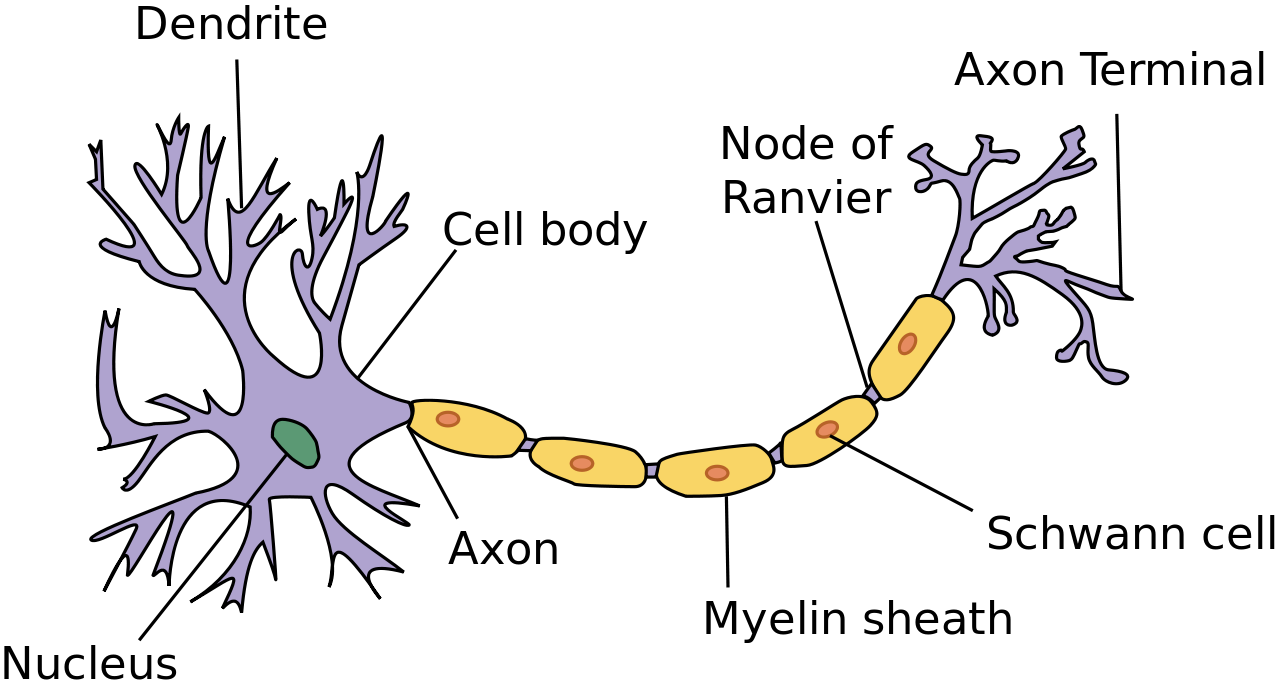
\includegraphics[scale=0.15]{./figure/human_neuron.PNG}\\

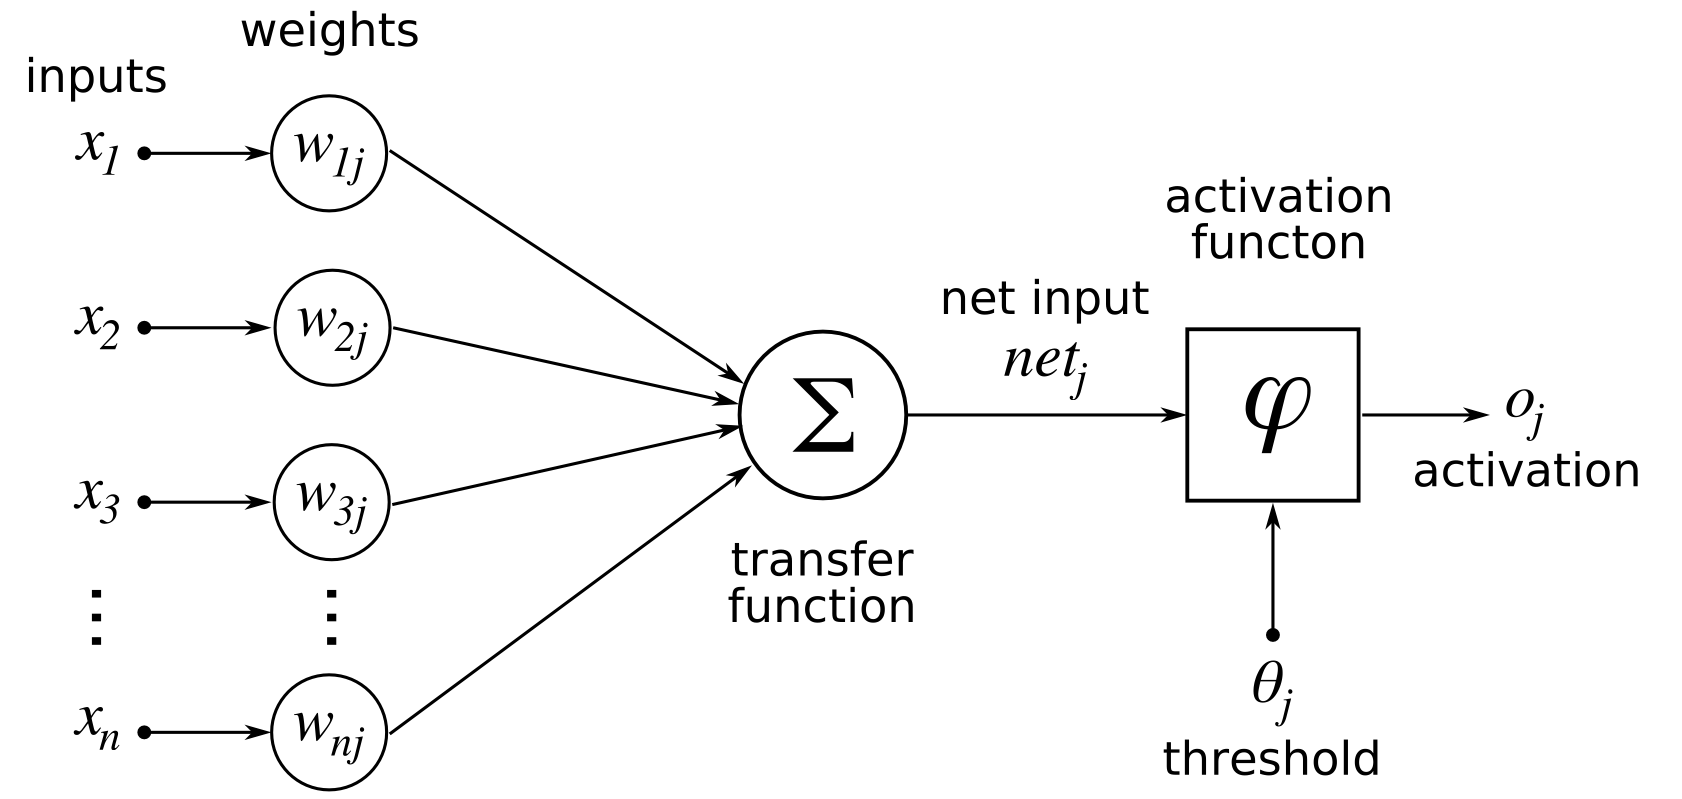
\includegraphics[scale=0.15]{./figure/nn_neuron.PNG}

\caption{A parallelism between a human-brain neuron and a neuron in a Brain Inspired Network\cite{WEBSITE:11}\cite{WEBSITE:13}}
\label{fig:neuron}
\end{figure}
In the human brain, the basic computational unit is the neuron.\\ Neurons receive input signal from dendrites and produce output signal along the axon which interacts with other neurons via synaptic weights.\\ The synaptic weights are obtained after a learning process, which can strengthen them or not.

\subsubsection{Neural Networks}

Neural Networks (or Artificial Neural Networks) are graphs in which every node is interconnected to others using edges, which have a weight properly tuned during the training process.\\
As mentioned before, each and every node of the neural networks is called artificial neurons (a loosely model of its biological counterpart) and the connections (synapses in biological brain) can transmit information from a neuron to another. In Figure \ref{fig:neuron} b the neurons receive signals, which is processed internally, and then they propagate it to the other connected neurons.\\
The information exchanged between a neuron and another is a real number, a result of a non-linear function of the sum of all its input.

In the Figure \ref{fig:nn} an implementation of a Neural Network can be appreciated.
\begin{figure}[H]
\centering
\captionsetup{justification=centering}
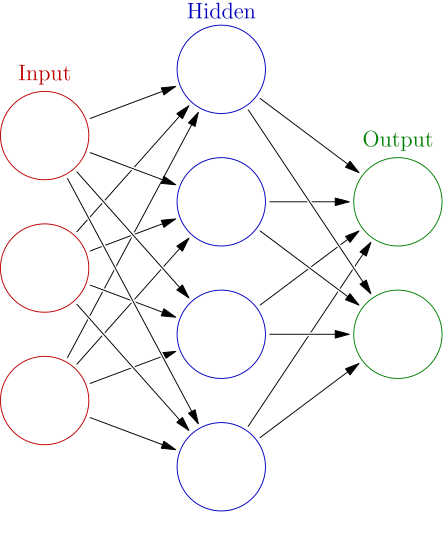
\includegraphics[scale=0.4]{./figure/neural_network.PNG}
\caption{Example of a Neural Network\cite{WEBSITE:10}}
\label{fig:nn}
\end{figure}
As it can be seen in Figure \ref{fig:nn}, it is always divided in layers in which only the output and input layers are visible from the external world, as consequence the internal layers are called hidden layers. When an input vector is applied, it will propagate from the left side of the network to its right side through the layers and the neurons which compose each layer. It is worth to mention that layers may perform different kind of computation on their inputs. Moreover, the deep neural networks are named after the huge amount of hidden layers.\\\\

In the early stages of ANNs the goal was to solve problems as the human brain would do. However, over time, the aim moved to perform specific tasks, leading to a different architecture of the biological brain and brain-inspired networks (Spiking Neural Networks).
\newpage
Depending on how the edges are connected and the topology, a Neural Network can be classified in several sub-types:
\begin{itemize}
\item Feedforward, the data move only from input layer to output layer without cycles in the graph.
\item Regulatory feedback, it provides feedback connections back to the same inputs that active them, reducing requirements during learning. It also allows learning and updating much easier.
\item Recurrent neural network, it propagates data backward and forward, from later processing stages to earlier stages.
\item Modular, several small networks cooperate or compete to solve problems.
\item Physical, it is based on electrically adjustable resistance material to simulate artificial synapses.
\end{itemize}

\subsubsection{Spiking Neural Networks}
Spiking neural networks (SNNs) are artificial neural networks that more closely mimic natural neural networks\cite{article:1}. \\In addition to neuronal and synaptic state, in their operational model, SNNs adds the concept of time. The idea is that neurons in the SNN do not activate at each propagation cycle but rather activate only when specific value is reached.\\
The current activation level is modeled as a differential equation and it is normally considered as neuron's state.

In principle, SNNs can be applied to the same application of Artificial Neural Networks. Moreover, SNNs can model brain of biological organisms without prior knowledge of the environment. Thus, SNNs have been useful in neuroscience for evaluating the reliability of the hypothesis on biological neural circuits but not in engineering.\\\\
SSNs are still lagging ANNs in terms of accuracy, but the gap is decreasing and has vanished on some task\cite{article:2}.
\newpage
\section{Machine Learning Quantization}
The reduction of computation demand and the increase of power efficiency of machine learning algorithms can be achievied through the quantization.\\\\

Quantization is basically a set of techniques which convert, and map, input values from a large set to output values in a smaller set.\\The idea of Quantization is not recent, it has been introduced since the birth of digital electronics. Imagine to take a picture with the phone's camera, the real world is analog and the camera is capturing the analog world and converting it into a digital format.  Nevertheless the high quality of nowadas pictures, quantization is not lossless.\\\\
\begin{figure}[H]
\centering
\captionsetup{justification=centering}
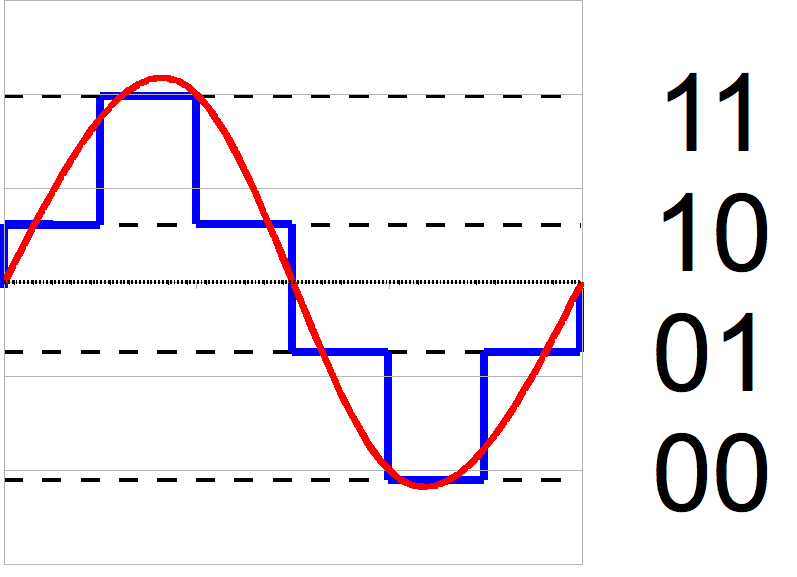
\includegraphics[scale=0.4]{./figure/quant.PNG}
\caption{Approximation of analog signal to digital signal\cite{WEBSITE:12}}
\label{fig:quant}
\end{figure}
Going back to machine learning, it has been proved that even if the model has been quantized, for example from fp32 to integer32, its accuracy is still good and the accuracy drop between the two data representation is negligible\cite{paper:8}. On the other hand, this quantization has lead to a relief of hardware computation, as it is very well-known floating point operation are much more expensive than integer operation from a lot of perspectives, and as consequence a reduction into the power consumptiom of the algorithm. It is also important to mention that the data traffic between the memory and the hardware is reduced due to the compaction of data.\\\\

Nowadays, edge devices take advantage of lower precision and quantized operations, including GPUs. Thus, Quantization of machine learning algorithms is a defacto standard for edge inference.

\section{Applications}
In principle the AI can be applied to any intellectual tasks. Focusing on machine learning applications, they can spread through a variety of different domains:
\begin{itemize}
\item Healthcare, mainly used for classification purposes.
\item Automotive, used in self-driving cars.
\item Finance and economics, to detect charges or claims outside the norm, flagging these for human investigation. In banks system for organizing operations, maintaing book-keeping, investing in stocks and managing properties.
\item Cybersecurity, automatically sort the data in networks into high risk and low-risk information.
\item Government, for paired with facial recognition systems may be used for mass surveillance.
\item Video games, it is routinely used to generate dynamic purposeful behavior in non-player characters.
\item Military, enhancing C2, Communications, Sensors, Integration and Interoperability.
\item Hospitality, to reduce staff load and increase efficiency.
\item Advertising, it is used to predict the behavior of customers from their digital footprint in order to target them with personalized promotions.
\item Art, it has inspired numerous creative applications including its usage to produce visual art.
\end{itemize}
However, all the Machine Learning applications are characterized by the need of a huge amount of data set for the training process.